\documentclass[10pt,a4paper]{report}

\usepackage[utf8]{inputenc}
\usepackage{amsmath}
\usepackage{amsfonts}
\usepackage{amssymb}
\usepackage{graphicx}
\usepackage{color}
\usepackage{lscape}
\usepackage{enumitem}
\usepackage[top=1cm, bottom=2cm, left=2cm, right=2cm]{geometry}
\usepackage{hyperref}
\usepackage{fancyhdr}
\pagestyle{fancy}

\fancyhead{}
\fancyfoot{} 
\lhead{ \hspace{0.1cm} M1 WI 2014-2015  \hspace{0.4cm} \vline}
\chead{Apprentissage automatique}
\rhead{K.B - B.B - K.L - N.R}
\rfoot{\thepage}

\author{Kevin BASCOL, Bachir BOUACHERIA, Kevin LAOUSSING, Nicolas REYNAUD}
\title{ Apprentissage automatique : Reconnaissance des formes}

\makeatletter
\renewcommand{\thesection}{\@arabic\c@section}
\makeatother

\begin{document}

\makeatletter
	\begin{titlepage}
	
	\centering
		{
		\vspace*{5cm}
		\hrule height 2pt
		\vspace{0.7cm}
		\Huge \textbf{\@title}}\\
		\vspace{0.7cm}
		\hrule height 2pt
		
		\vfill
		\vspace{1cm}
		\@author\\
		\end{titlepage}
\makeatother
\setcounter{secnumdepth}{4}
\setcounter{tocdepth}{3}
\renewcommand{\contentsname}{Sommaire}
\begingroup\makeatletter
\def\@makeschapterhead#1{%
  {\parindent \z@ \raggedright
    \normalfont
    \interlinepenalty\@M
    \Huge \bfseries  #1\par\nobreak
    \vskip 20pt% <---- à réduire pour avoir plus de place
  }}\makeatother
\tableofcontents
\endgroup
\thispagestyle{empty}
\setcounter{page}{0}
\newpage

\newgeometry{top=2cm, bottom=2cm, left=2cm, right=2cm}

%%%%%%%%%%%%%%%%%%%%%%%%%%%%%%%%%%%%%%%%%%%%%%%%%%%%%%%
%%%					INTRODUCTION					%%%
%%%%%%%%%%%%%%%%%%%%%%%%%%%%%%%%%%%%%%%%%%%%%%%%%%%%%%%
\section{Introduction}
\begin{flushleft}

La reconnaissance de formes est une branche de l'intelligence artificielle qui fait appel aux techniques d'apprentissage automatique. Durant ce projet, nous avons réalisé un logiciel de reconnaissance de formes, où les formes sont les nombres de 0 à 9.
La réalisation comprend la développement d'une interface graphique ergonomique facilitant la construction d'une base d'apprentissage, la manipulation des algorithmes d'apprentissage et la visualisation des résultats des tests d'apprentissage. Et elle comprend aussi l'implémentation de deux méthodes d'apprentissages : les k-plus-proches voisins, et le réseau de neurones.\\
Dans un premier temps nous allons présenter notre organisation autour de ce projet. Puis dans un deuxième temps, nous décrirons les fonctionnalités de notre logiciel. Nous présenterons par la suite les résultats et les performances de notre logiciel à la reconnaissance des nombres.\\
Enfin nous terminerons par une conclusion qui résumera l'efficacité des algorithmes.


\end{flushleft}


%%%%%%%%%%%%%%%%%%%%%%%%%%%%%%%%%%%%%%%%%%%%%%%%%%%%%%%
%%%					ORGANISATION					%%%
%%%%%%%%%%%%%%%%%%%%%%%%%%%%%%%%%%%%%%%%%%%%%%%%%%%%%%%

\section{Organisation du projet}

\subsection{Planning}
\begin{flushleft}
Le planning prévisionnel et le planning final sont disponibles en annexe.
\end{flushleft}



%%%%%%%%%%%%%%%%%%%%%%%%%%%%%%%%%%%%%%%%%%%%%%%%%%%%%%%
%%%					FONCTIONNALITES				%%%
%%%%%%%%%%%%%%%%%%%%%%%%%%%%%%%%%%%%%%%%%%%%%%%%%%%%%%%

\section{Fonctionnalités}

\subsection{Interface graphique}
\begin{figure}[!h]
	\center
		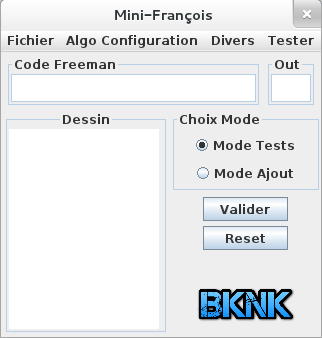
\includegraphics[scale=0.5]{./Ressource/IG.png}
 	\caption{Interface graphique de Mini-François}
\end{figure}

\subsubsection{Module de saisi de données}
\begin{flushleft}
Pour interagir avec le logiciel nous avons développé un module de saisi possédant deux modes : un mode permettant de générer des données pour créer la base d'apprentissage, et un mode pour tester notre système.\newline \newline
Le module est composé de :

\begin{itemize}[label=$-$,leftmargin=*,parsep=0cm,itemsep=0.1cm,topsep=0cm]
\item un canevas de dimension de 200x150 pour dessiner un chiffre à la souris.

\item un champ de texte "out/in" dans lequel on indique le chiffre qu'on dessine dans le canevas.

\item un autre champ de texte "code de freeman" dans lequel apparaît le code freeman du chiffre dessiné.

\item un groupe de deux radio-boutons pour sélectionner le mode du module de saisi.

\item un bouton "Valider" pour valider l'acquisition de la donnée (en mode ajout) et pour lancer le test (en mode test).
\item un bouton "Reset" pour annuler l'acquisition de la donnée en cas d'erreur. Le bouton reset remet a zero les champs du Code de freeman, le champs "Out/In" suivant le mode, et vide la zone de dessin.
\end{itemize}

\end{flushleft}

\begin{figure}[!h]
	\center
		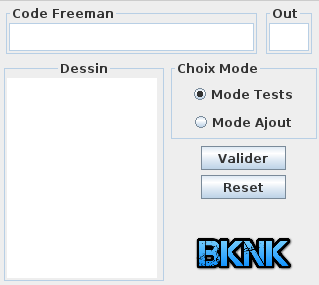
\includegraphics[scale=0.5]{./Ressource/Module_saisi.png}
 	\caption{Module de saisi de données}
\end{figure}

\paragraph*{Mode test}
\begin{flushleft}
Si le radio bouton "Mode Test" est sélectionné alors le logiciel lance l'algorithme avec les paramètres spécifiés dans le menu "Algo configuration" et le chiffre dessiné dans le canevas.
\end{flushleft}


\paragraph*{Mode ajout}
\begin{flushleft}
Si le radio bouton "Mode Ajout" est sélectionné alors le logiciel enregistre le code de freeman et la matrice correspondant au chiffre dessiné dans le canevas dans un fichier "Base" correspondant à la base d'apprentissage du logiciel.

En mode Ajout un bouton viens de rajouter à l'interface graphique, et le champs "Out" deviens un champs "In".

\item Le bouton ajouté est le bouton "Revert" : Si on dessine un chiffre A dans le canevas mais qu'il ne correspond pas au chiffre B entré dans le champ de texte "In" et qu'on a valider l'acquisition par mégarde, il est possible d'annuler l'acquisition grâce au bouton "Revert" qui aura pour action de supprimer la dernière entrée de la base.

\end{flushleft}

\subsubsection{Module de configuration}

\begin{flushleft}
Le module de configuration permet de renseigner les paramètres de nos algorithmes. Il est accessible à partir du menu "Algo Configuration".\\
On peut cocher l'algorithme (ainsi que les paramètres qu'on souhaite utiliser") que le logiciel doit utiliser en "mode test". 
\end{flushleft}

\subsubsection{Module de visualisation statistique des données d'apprentissages}
\begin{flushleft}

Le module de visualisation statistique des données d'apprentissage nous permet d'évaluer la progression d'apprentissage de notre système à travers divers graphiques :

\begin{itemize}[label=$-$,leftmargin=*,parsep=0cm,itemsep=0.1cm,topsep=0cm]

\item un histogramme représentant l'état de la base d'apprentissage (nombre d'exemples par chiffre).

\item un histogramme représentant le nombre de résultats juste/faux par chiffre pour un jeu d'exemple de test donné.

\item un camembert indiquant la précision des résultats pour un jeu d'exemple de test donné.

\item un histogramme indiquant le nombre de résultats juste/faux pour chaque algorithme, avec le même jeu d'exemple de test donné.

\end{itemize}

\end{flushleft}

\subsection{Algorithmes d'apprentissage}

\subsubsection{Base d'apprentissage}

\subsubsection{Algorithme k-PPV}
l'utilisation de l'algorithme des k plus proches voisins, consiste à résoudre la problématique en utilisant des distances.
dans notre application, on a utilisé 4 distances différentes qui sont : 
\begin{itemize}[label=$-$,leftmargin=*,parsep=0cm,itemsep=0cm,topsep=0cm]
\item Distance euclidienne
\item Distance de Manhattan 
\item Distance de Chebyshev
\item Distance d'édition(où de Levenshtein)
\end{itemize}
tel que l'algorithme utilise les 3 premières distances pour comparer des matrices entre elles, alors que la distance d'édition est utilisé pour trouver la distance entre deux chaines de code de Freeman qui représentent le chiffre.
Après plusieurs essais, on a constaté que l'algorithme des k plus proches voisins est plus performant quand on utilise la distance d'édition (code de Freeman), contrairement à l'utilisation de la distance de Chebyshev.
quant à l'utilisation de nombre différent de voisins (3-ppv, 5-ppv et 7-ppv), on constate qu'il n'y a pas une grande différence entre les taux de réussite.

\subsubsection{Algorithme réseau de neurones}
\begin{flushleft}

Pour le réseau de neurones, comme nous étions en retard, nous avons choisi d'utiliser une implémentation déjà faite sur internet. Nous avons choisit d'utiliser celle de WEKA comme nous avions déjà eu un aperçu pendant la séance de TP.\\
\vspace*{0.3cm}
Tout d'abord nous avons tenté d'utiliser comme entrée la matrice. Comme nous utilisons une matrice de 150x200 celle-ci donnerait un nombre trop conséquent de pixel à passer en entrée. Nous avons donc réduit la matrice à l'aide d'une matrice 10x10 ce qui a réduit le nombre d'entrée à 300. Pour effectuer la réduction nous sommons les valeurs contenues dans la matrice 10x10 et remplissons alors la nouvelle matrice avec ces valeurs (on utilisait donc pas une matrice binaire).\\
Nous avons effectué de nombreux tests avec différentes variantes de couches et de learning rate. Avec cette méthode nous avons réussi à atteindre un taux de réussite de 80\% maximum, ce qui était relativement satisfaisant par rapport aux autres algorithmes utilisant la matrice comme entrée.\\
\vspace*{0.3cm}
Ensuite nous avons essayé d'utiliser comme entrée le code de freeman. Pour le code de freeman le problème est d'arriver à obtenir un nombre d'entrées constant. La première idée à été de compter le pourcentage d'occurrence de chaque vecteur de freeman, mais cette méthode c'est avérée trop peu restrictive et fournissait un taux de réussite inférieur à 30\%.\\
Il nous fallait donc trouver une meilleure méthode. nous avons alors eu l'idée de diviser le code de freeman en plusieurs parties, ceci a pour effet d'éviter les chiffres qui ont la même proportion de vecteur de freeman mais pas aux même endroits. Nous avons alors testé de faire le pourcentage d'occurrence de chaque vecteur dans chaque partie. Diviser en 2 a permis de passer à plus de 50\% de réussite, en 4 à 83\%, en 6 à 93\% de même pour 8 qu'on utilise donc maintenant. Après quelques modifications de learning rate et de couches nous avons réussi à atteindre un taux d'un peu plus de 94\%.\\
Nous avons donc conservé cette configuration pour notre réseau de neurone final.

\end{flushleft}


%%%%%%%%%%%%%%%%%%%%%%%%%%%%%%%%%%%%%%%%%%%%%%%%%%%%%%%
%%%						ETUDE						%%%
%%%%%%%%%%%%%%%%%%%%%%%%%%%%%%%%%%%%%%%%%%%%%%%%%%%%%%%

\section{Etude}

\subsection{Description de la fonctionnalité}
\begin{flushleft}
•
\end{flushleft}

\subsection{Description technique}
\begin{flushleft}
•
\end{flushleft}


%%%%%%%%%%%%%%%%%%%%%%%%%%%%%%%%%%%%%%%%%%%%%%%%%%%%%%%
%%%						CONCLUSION					%%%
%%%%%%%%%%%%%%%%%%%%%%%%%%%%%%%%%%%%%%%%%%%%%%%%%%%%%%%

\section{Conclusion}
\begin{flushleft}
•
\end{flushleft}


%%%%%%%%%%%%%%%%%%%%%%%%%%%%%%%%%%%%%%%%%%%%%%%%%%%%%%%
%%%						ANNEXES						%%%
%%%%%%%%%%%%%%%%%%%%%%%%%%%%%%%%%%%%%%%%%%%%%%%%%%%%%%%

\section{Annexe}
\subsection*{Sources}
\begin{description}
	\item[WEKA] \url{http://weka.sourceforge.net/doc.dev/overview-summary.html}
\end{description}
\newpage

\begin{landscape}
\subsection*{Planning}

\begin{figure}[!h]
	\center
		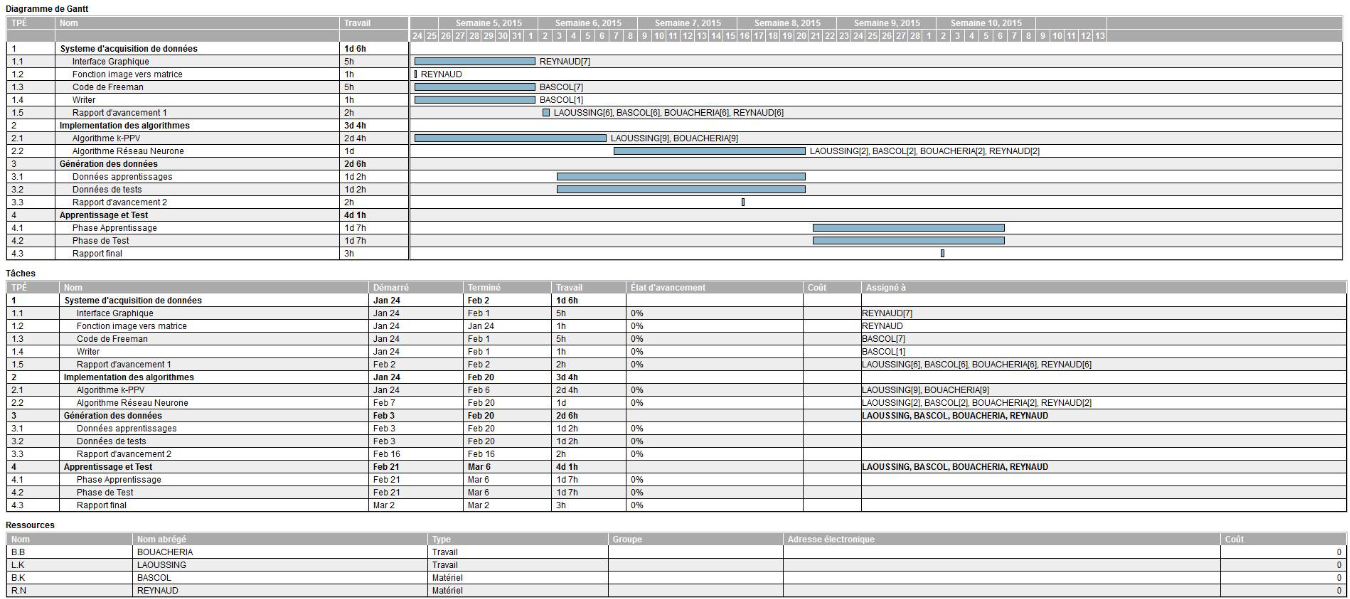
\includegraphics[scale=0.5]{./Ressource/planning_previsionnel.png}
 	\caption{planning au prévisionnel 19/01/15}
\end{figure}
\newpage
\subsection*{Planning}
\begin{figure}[!h]
	\center
		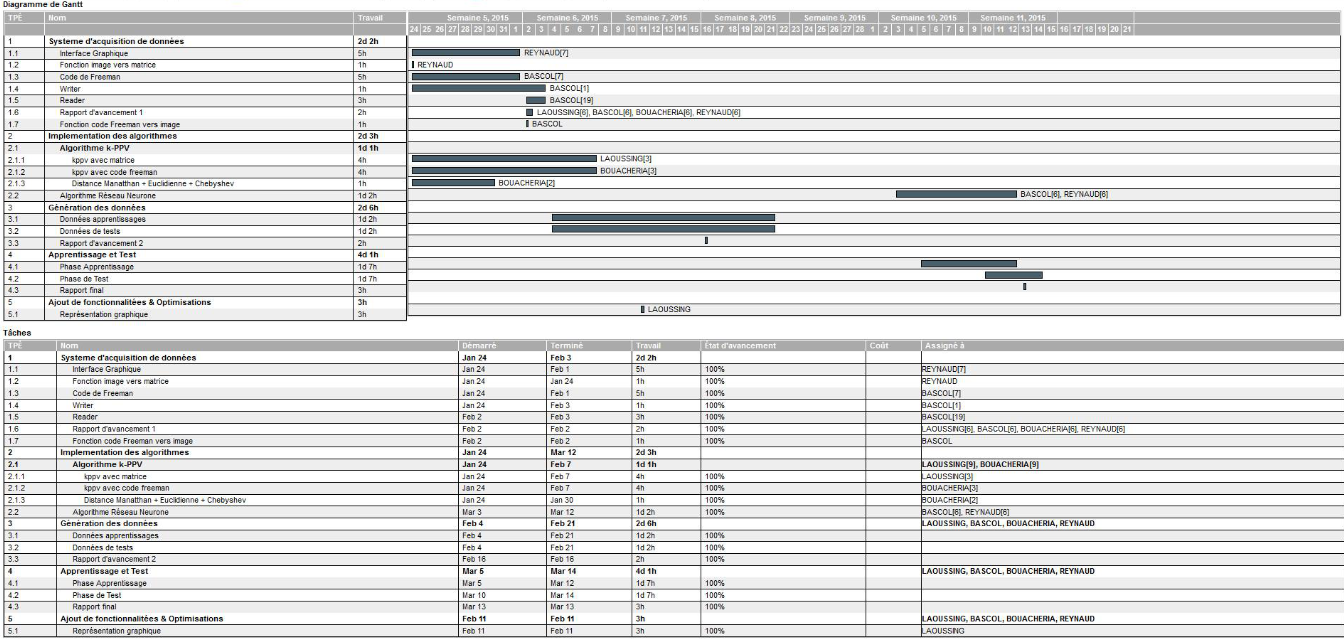
\includegraphics[scale=0.5]{./Ressource/planning_final.png}
 	\caption{planning final 05/03/15}
\end{figure}
\end{landscape}
\end{document}
